\documentclass[11pt,a4paper]{article}
\usepackage[margin=25mm]{geometry}
\usepackage[T1]{fontenc}
\usepackage[utf8]{inputenc}
\usepackage{lmodern,amsmath,amssymb,booktabs,enumitem,graphicx,microtype,multirow}
\usepackage[section]{placeins}
\usepackage{tabularx,longtable,xcolor,xurl}
\usepackage[hidelinks]{hyperref}
\usepackage[nameinlink,noabbrev]{cleveref}
\hypersetup{pdftitle={Review-to-Execution Continuity - Supplementary Material},pdfauthor={Liang Hanghao; Xuan Wentao; Chen Qile; Peng Peng},pdfsubject={Correction-aware review-to-execution continuity, authorization and agent recovery}}
\setlength{\emergencystretch}{2em}
\newcommand{\system}{\textsc{Auto-Decte}}
\newcommand{\code}[1]{\nolinkurl{#1}}
\newcommand{\eqc}{\mathrel{=_{\mathrm{json}}}}
\newcommand{\neqc}{\mathrel{\neq_{\mathrm{json}}}}

\renewcommand{\thesection}{S\arabic{section}}
\renewcommand{\thetable}{S\arabic{table}}
\renewcommand{\thefigure}{S\arabic{figure}}
\begin{document}
\begin{center}
{\Large Online Resource 1}\par\medskip
{\large Review-to-Execution Continuity for Corrected Agent State Changes}\par\medskip
Liang Hanghao, Xuan Wentao, Chen Qile, and Peng Peng
\par\smallskip{\small Knowledge and Information Systems\\College of Computer Science and Electronic Engineering, Hunan University, Changsha, China\\Corresponding author: Peng Peng, \texttt{hnu16pp@hnu.edu.cn}}
\end{center}

This supplement retains the archived formal, implementation, controlled-workload and historical integration details, and adds the prospective policy design and collection rules. The archived evidence layers, completed original prospective ledger and incomplete supplementary quota-recovery cohort remain separately identified. Sections, tables and figures prefixed S belong to this document. The complete original prospective ledger and result tables retain terminal failures and unknown coverage on the original planned denominator. The separately frozen quota-recovery snapshot is documented in Section S12 and contributes no observations to the original analysis.

\paragraph{Reading guide.} For the execution contract and formal assumptions, start with Sections S2--S3. Sections S1 and S4--S7 preserve the controlled and historical evidence. Sections S8--S9 define the online design and reproducibility procedures; Section S11 contains the complete original results. Section S12 states exactly what remains pending for supplementary recovery. The main manuscript provides the scientific narrative and four overview figures.

\section{Artifact, protocol, and reproduction}
\label{app:artifact}

\subsection{Three evidence layers}

The reference implementation is fixed at commit \code{c6d512843c905cab6d8521dd8c914f7fb26d85ae} of \url{https://github.com/lhh666-6/auto-dete}, using \code{latest/code/implementation-fixed}. The tag \code{r31-jss-2026-09-13} retains formal models, observation witnesses, repaired code, and historical analyses. The historical v8 evidence remains under \code{r21-jss-2026-09-07-v8}. These layers are not substituted for one another when reporting counts or timings.

The new E1--E3 package is fixed at \url{https://github.com/lhh666-6/auto-dete/tree/2645e5e18c900ea91c9c980e44195dc71e410432/DKE-supplement}. Its \code{PROTOCOL.md} was drafted before outcome collection on 23 September 2026 and records pilot-driven amendments. It is a local prospective execution plan, not an externally registered protocol. Pilots remain in separately named directories and are excluded from final statistics. No hosted-model call was made in E1--E3.

\begin{table}[htbp]
\centering\small
\caption{New experiment evidence and interpretation units. Paths are relative to the pinned \code{DKE-supplement} directory.}
\begin{tabularx}{\textwidth}{@{}l>{\raggedright\arraybackslash}p{0.40\textwidth}X@{}}
\toprule
Layer & Primary records & Unit and limit \\
\midrule
E1 & \code{results/e1/inputs.json}; \code{results/e1/receipts.jsonl} & 495 constructed executions; 165 per arm; seven distinct proposal values. \\
E2 & \code{results/e2/browser-observations.jsonl}; screenshots and databases & 60 scripted cases plus six replay setup confirmations; not a human study. \\
E3 & \code{results/e3/*/raw.jsonl}; \code{summary.json}; \code{paired.json} & 22,400 timed observations, excluding warmups; one machine. \\
Checks & \code{rejection-audit.json}; \code{verification.json}; \code{regression-receipt.json} & Expected rejection causes, counts, state digests, and test execution receipt. \\
Integrity & \code{artifact-manifest.json}; \code{source-integrity.json} & Content identities, not third-party attestation. \\
\bottomrule
\end{tabularx}
\end{table}

\subsection{Inputs, cases, and negative controls}

E1 selects the first lexicographically ordered archived run containing a proposal in each of the G1/G2/D1 by B1--B4 cells; success labels are not a selection criterion. The twelve cells contain four distinct proposed values: 8, 100, the string \code{B-008}, and 9. Three additional controls exercise $2\rightarrow2.0$, $1\rightarrow\mathrm{true}$, and nested integer/float changes. These values enter newly constructed form histories with fresh certificates and review records. This is not an end-to-end replay of the original tasks. Input records retain source paths, event identifiers, and hashes.

The eleven cases per input are Accept, Correction, multi-field admission, equal-valued candidate substitution, different-evidence substitution, stale authorization, replay, an unauthorized submitted value, and interruptions after CAS, before transition insertion, and before commit. The rich-context journal retains field, version, evidence, producer and proposal context, but its review projection excludes certificate identity, candidate identifier, and instance creation time. Its exact variant adds the reviewed-candidate link. Each successful three-field record is checked with six queries per field: proposed value, authorized value, reviewer, reviewed candidate, current value, and source version. The 18 answers per accepted case are query observations, not independent experiments.

E2 uses the JSON values 100, 2.5, and true. Each appears in ten interactions per path: Accept, Correction, legitimate reselection, candidate-request substitution, authorized-value substitution, principal substitution, stale state, replay, precommit interruption, and display-only substitution. The driver records DOM candidate identity, proposal, and authorized value before confirmation. Replay cases each require an initial confirmation, explaining the six additional setup calls. The float value 2.5 avoids JavaScript serialization normalizing an integral float to an integer. The gate records a server-held review session using fixed simulated principal labels and a database separate from the fact database.

The rejection audit checks all 372 rejected attempts across E1 and E2, including their exact expected error categories or injected failpoints. No rejected attempt changes the measured fact-database digest. The baseline is taken after authorization preparation: already recorded review intent is not required to disappear when admission fails. This distinction also prevents the session database from being silently included in a fact-database atomicity claim.

\subsection{Execution environment and commands}

The recorded environment is Intel Core i7-10875H, Windows 10 build 19045, CPython 3.11.16, SQLite 3.53.1, and SQLAlchemy 2.0.51. Browser orchestration uses Playwright and local Chrome. E3 uses a seeded random ordering of the two arms (seed 20260923), five warmups, and 200 timed observations per arm and cell. Admission uses SQLite DELETE/FULL; the storage-population measurement uses WAL/NORMAL followed by checkpointing. Background operating-system activity was not controlled.

The deposited README specifies dependency installation, reference-source resolution, and the separate browser driver environment. The following commands illustrate the entry points; the output directory must be fresh, and the reference checkout must be configured as described there. Performance should run after other tests have finished.
\begin{quote}\small\ttfamily
python -B experiment1.py -{}-output results/replicate-e1\par
python -B experiment2.py -{}-output results/replicate-e2\par
python -B experiment3.py -{}-output results/replicate-e3
\end{quote}
Pilot flags reduce coverage and cannot reproduce final denominators. The reference regression invocation covers its value-equality integration tests and conformance directory (85 passes); the supplementary test module records ten passes. The regression receipt transcribes the execution tool output rather than presenting itself as a pytest-generated JUnit report. The manifest records 61 pre-run measurement-source hashes; the reporting check found them unchanged. The original artifact manifest covers 3,068 files.

\subsection{Lossless storage packaging}

The 100,000-transition full database is 141,062,144 bytes and is published as \code{results/e3/storage/storage-100000/full.db.gz}. The publication package includes \code{restore_large_database.py} and \code{publication-packaging.json}. Restoration checks the uncompressed SHA-256 against the original manifest; its verified value is
\begin{quote}\small
\code{a6ab45b86b3f198e8452b7adae756012807efe09ceb92d32c759cd9d2ffb816e}.
\end{quote}
Compression changes transport size, not the database footprint used in the storage result. The restoration helper refuses to overwrite a differing existing file. Source and artifact manifests support reproducibility checks; they do not establish external validity or independent replication.

\section{Formal and implementation evidence}
\label{app:formal-details}

\subsection{Complete observation functions and witness construction}

Main Section 3 gives the observation basis, opaque-handle condition, outcome definition, Proposition 1 and its paired-history construction. The following table and relational representation specify the complete executable projection.
\begin{table}[t]
\centering
\footnotesize
\caption{Observation functions used by the conditional characterization. ``Derives'' lists information available without consulting another class.}
\label{tab:observation-functions}
\begin{tabularx}{\textwidth}{@{}l>{\raggedright\arraybackslash}p{0.28\textwidth}>{\raggedright\arraybackslash}p{0.25\textwidth}>{\raggedright\arraybackslash}X@{}}
\toprule
Class & Raw history components exposed & Derives & Deliberately excludes \\
\midrule
$D_C$ & opaque candidate and authorization-target handles; candidate and admission targets; field, evidence, producer & candidate binding and non-temporal context agreement & decoded proposal/authorized values, current version, batch-effect domain, successor sources \\
$D_V$ & proposal value, authorized value, committed value, and their role labels for an anonymous batch item & Accept versus Correction and proposal/authority attribution & candidate handle and context, temporal order, batch completeness, source identities \\
$D_F$ & expected and transactionally observed pre-state discriminator at the admission attempt & current versus superseded authorization & proposal roles, non-temporal candidate context, batch effects, source relation \\
$D_B$ & declared item-field domain, committed effect domain, commit grouping, and successor count & complete versus partial/fragmented successor construction & value-role attribution, freshness, and field-source identities \\
$D_S$ & successor field--source relation; local resolution and copy-forward checks & missing/ambiguous sources, field/value inconsistency, and replaced unchanged sources & commit grouping, value roles, freshness, and candidate context \\
\bottomrule
\end{tabularx}
\end{table}

For the executable construction below, each finite history is represented by the complete tuple
\begin{equation}
\widehat h=\langle r,C,A,B,v_{\mathrm{exp}},v_{\mathrm{obs}},
F_{\mathrm{decl}},K,V_v,V_{v'},S_v,S_{v'},T\rangle,
\label{eq:witness-history}
\end{equation}
containing the target, candidate and authorization registries, batch references, expected and observed pre-versions, declared fields, a commit sequence $K$, endpoint value and source maps, and a registry $T$ of source-transition identifiers, fields, and values. Each commit step records a distinct successor identity and complete before/after value maps. The domain predicate checks unique candidate and authorization keys, resolvable batch references, schema-valid fields, total value maps, and a connected commit sequence from $V_v$ to $V_{v'}$. Its committed effect domain is the union of the steps' actual value-change domains; its successor count is $|K|$. Neither is an independently assigned witness attribute.

Source observations expose each field's anchor count, reverse-resolution count in $T$, agreement of the resolved field/value with the successor, and exact prior-source retention for an unchanged field. Missing, duplicate, or inconsistent sources remain semantic failures rather than being excluded by the domain predicate. These are local source checks: the complete authorization--candidate--evidence chain belongs to the operational P6 checks defined below. Source observations hide intermediate commit grouping; freshness observes the admission-entry pre-state comparison. These explicit observation boundaries make it possible to compare atomic and fragmented histories with identical endpoints.

Main Section 3 states Proposition 1, summarizes the five paired-history constructions and gives the reduced-projection equation. The original candidate/context witness changes record context with a fixed candidate handle. The separate identity-isolation pair fixes the two-candidate registry and the non-identity observations, then changes the admitted candidate. The executable checker derives outcomes and observations from the complete tuple rather than storing either as an independent attribute.

\subsection{Evidence identity and operational enforcement details}
Evidence identity is not content equality alone. The realization uses
\begin{equation}
EID(e)=\langle H(\mathrm{bytes}(e)),L(r,f,u,\kappa)\rangle,
\label{eq:evidence}
\end{equation}
where $H$ is SHA-256 and $L$ is a versioned canonical locator containing the owner record, related field, normalized storage-relative URI $u$, and optional crop identity $\kappa$. The Alloy model abstracts content and locator as primitive domains. Its \code{certIdentityFacts} assigns distinct \code{CertId} atoms to distinct certificate objects, including objects with equal modeled content. Relating this abstraction to the implementation requires collision resistance of the deployed digest and integrity of the canonicalization and evidence store; it is not a proof or claim that SHA-256 is mathematically injective.

\paragraph{Full operational contract.}
Table~\ref{tab:s-contract} defines the operational properties referred to by the formal and implementation evidence. Main Sections 3--4 retain the role definitions and executable realization.
\begin{table}[htbp]
\centering\small
\caption{Operational contract for a corrected authoritative transition.}
\label{tab:s-contract}
\begin{tabularx}{\textwidth}{@{}l>{\raggedright\arraybackslash}p{.25\textwidth}X@{}}
\toprule
Property & Requirement & Operational interpretation \\
\midrule
P0 & Direct-write exclusion & Candidate-writing capability cannot change authoritative values, versions, sources, transitions or authorizations. \\
P1 & Instance binding & Authorization refers to the canonical persisted candidate certificate, including instance identity. \\
P2 & Context integrity & Record, field, persisted evidence content and locator, and expected predecessor agree across the item and certificate. \\
P3 & Authorization integrity & The principal is allowed at the in-transaction check, and the authorization fixes the certificate and explicit committed value. \\
P4 & Freshness & The expected predecessor equals the transactionally observed current version; stale or competing admissions are rejected. \\
P5 & Successor integrity & One atomic successor has exact changed-field effects, an item--transition bijection and complete unchanged-field framing. \\
P6 & Trace soundness & Every field resolves through its exact source transition to consistent authorization, candidate, evidence, producer and version relations. \\
\bottomrule
\end{tabularx}
\end{table}

\paragraph{Admitted effects and no-op semantics.}
After initial coverage, concrete admissions require a nonempty value change under canonical JSON equality. For submitted items $U$, the admitted batch is $B=\{i\in U\mid i.x\neqc V_v(i.f)\}$, with $B\ne\varnothing$. All items in $B$ share one record and expected predecessor and have unique changed fields. A mixed submission admits exactly $B$; unchanged items retain their exact preceding source and create no new transition or authorization binding. Initial coverage establishes a complete value and source domain. The Alloy model additionally permits same-value admission for correspondence with the historical singleton model. A renewed review or re-attribution without a value change uses a separate review-event path, outside the concrete admission contract.

The trusted base includes the admission service, exercised transaction semantics, canonicalization, hashing and principal policy. Authentication, review presentation and evidence storage must supply the identities and content on which those checks operate. Rejection stutters relative to authoritative state immediately before the admission attempt; it need not erase evidence, candidate preparation or review intent persisted earlier.

\paragraph{Authorization timing and revocation}
\label{app:authorization-timing}
The prototype evaluates the in-memory principal-role allow-list inside the database transaction, before the version compare-and-swap and any authority write. A revocation that completes before this check causes zero-write rejection. The allow-list lock protects only the policy lookup/update; it is not held for the remainder of the database transaction. Consequently, a revocation that overlaps an admission after its successful policy check does not cancel that in-flight commit. The implementation therefore provides commit-entry revalidation, not linearizable revocation against already admitted operations, distributed identity-provider semantics, or session invalidation. Deployments requiring those properties must place a transactional policy epoch or equivalent revocation discriminator inside the admission compare-and-swap.

Human authorization is not a truth oracle. The contract establishes who authorized which persisted candidate and value in which context, and whether the successor was constructed atomically. It cannot establish that the authorized value is factually correct.




\subsection{Information-class and persisted-state mappings}
Table~\ref{tab:distinction-evidence} connects each information class to its failure witness and executable evidence. Table~\ref{tab:abstraction} records how persisted relations are represented in the concrete/formal projection.
\begin{table}[t]
\centering
\footnotesize
\caption{Mapping from failure-distinguishing information classes to bounded and concrete evidence.}
\label{tab:distinction-evidence}
\begin{tabularx}{\textwidth}{@{}l>{\raggedright\arraybackslash}p{0.28\textwidth}>{\raggedright\arraybackslash}p{0.29\textwidth}>{\raggedright\arraybackslash}X@{}}
\toprule
Class & Safe/unsafe witness & Alloy support & Concrete support \\
\midrule
$D_C$ & matching / mismatched non-temporal candidate context; separate equal-valued identity-isolation pair & field, evidence-identity, evidence-owner, record, authorization-certificate, certificate-preexistence, and evidence-preexistence ablations & record, field, evidence, and certificate substitution cases \\
$D_V$ & retained Correction / wrong attribution of the same final value & legal Correction witnesses and authorization-value ablation & singleton, all-field, and mixed Correction lifecycles with immutable candidate checks \\
$D_F$ & current / superseded authorization & certificate-version and freshness ablations; stale-rejection assertions & stale replay, contending confirmation, and compare-and-swap rejection \\
$D_B$ & atomic / partial or fragmented successor & transition-bijection ablation and whole-batch framing assertions & exact changed-field validation, failpoints, rollback, and concurrency cases \\
$D_S$ & complete / missing, replaced, or duplicate source & source-anchor attack witnesses and P6 trace assertions & source-corruption catalogue and reverse-trace validation \\
\bottomrule
\end{tabularx}
\end{table}

\begin{table}[t]
\centering
\caption{Principal elements of the executable abstraction.}
\label{tab:abstraction}
\begin{tabularx}{\textwidth}{@{}>{\raggedright\arraybackslash}p{0.25\textwidth}>{\raggedright\arraybackslash}p{0.29\textwidth}>{\raggedright\arraybackslash}X@{}}
\toprule
Persisted relation & Formal relation & Mapping condition \\
\midrule
form and declared fields & Record and authoritativeFields & one target record with an exact selected field domain \\
evidence row plus locator & Evidence content and locator & owner/content/canonical persisted locator remain separate dimensions \\
candidate-certificate row & Candidate, Certificate, CertId & target, field, evidence, version, value, producer, and identity fixed \\
decision plus binding & Authorization & principal, certificate, and explicit authorized value fixed \\
record-version values & committedValue & complete canonical JSON equality classes in pre and post \\
record-version fact\_sources & committedSource & exact persisted transition atom per authoritative field \\
transition rows at successor & AdmissionItem transitions & exact item--transition set and complete relation fields \\
current-version/CAS unit & BatchAdmissionEvent envelope & one record, principal, pre-version, successor, and atomic pre/post \\
\bottomrule
\end{tabularx}
\end{table}

\subsection{Legal, unsafe, and preservation commands}

Six legal-witness commands cover multi-field Accept, Correction, mixed Accept/Correction, same-value admission, initial snapshot, and singleton admission. Eleven paired ablations remove the conjuncts mapped in Table~\ref{tab:distinction-evidence}. Principal membership remains fixed; the unused \code{ABL\_7} marker is excluded because host identity trust is an external assumption.

Three source-attack commands start from a legal Full prefix and then remove a source anchor, replace it, or add a duplicate source-version transition; each requires an incomplete trace. Fourteen assertions run per scope. Nine guard definitions and immediate consequences: P0/P1/P3/P4/P5, whole-batch effects, rejection framing, and two P6 checks. Five check invariant preservation, two singleton correspondences, rejection of an ablated attempt, and positive trace completeness under a well-formed pre-state.

The positive assertion requires a trace-complete predecessor and no stray transition to the successor version; otherwise the permissive base effect admits a post-state that fails \code{traceComplete}. It covers admitted fields in one step, not arbitrary histories or every carried-forward field. Both profiles include reachable initial and non-vacuous carry-forward witnesses for the precondition. Removing the post-state certificate binding changes UNSAT to SAT. These are separate checks of reachability, bounded preservation, and sensitivity, rather than fourteen independent proofs. Concrete enforcement additionally validates predecessor prefixes and uses transition uniqueness and in-transaction CAS revalidation.

\subsection{Scopes and interpretation}

The S1 profile bounds principal structural domains at two records, three fields, six versions, up to six admission items/transitions for most commands, and four states/events. S2 increases representative bounds to three records, four fields, eight versions, up to eight admission items/transitions, and five states/events. Individual commands adjust Value, Evidence, or Transition bounds when a witness needs an extra atom. The artifact contains the executable scopes; this summary is not a replacement for them.



An UNSAT assertion means that the Analyzer found no counterexample within the encoded command scope. A SAT run means that it found the requested witness; the main text cites the Analyzer and solver references. Singleton contract/effect checks additionally guard the batch lift against silently changing the historical one-item semantics.


\subsection{Observation witnesses and finite scopes}

The executable witness checker derives observations and outcomes from complete relational histories. Five class pairs test Proposition 1; a further pair isolates instance identity with a fixed two-candidate registry, and a legal control changes one field while copying another field's exact source. The original source is \code{latest/code/formal-fixed/observation_witnesses.py}, with report \code{latest/evidence/r27-witness/observation-witness-report-v5.json}. The handoff also includes the repaired executable construction and 24 tests under \code{research/authorization-granularity-phase1-2026-10-06/formal/}.

Across the two scope profiles, the archived command manifest records 72 expected matches: 22 SAT and 14 UNSAT per profile. Sections S2.4--S2.5 define their commands, premises and scope interpretation. The independent projection outcomes and concrete checks below provide a separate check of the implementation-to-model boundary.

\subsection{Projection and database oracles}

The projection adapter reads persisted pre/post state independently of the production planner and trace builder, maps JSON equality classes and identity relations into a fixed Alloy instance, and checks committed or rejected wrappers. Nine intended instances are SAT and twenty selected mapping mutants are UNSAT. A rejected wrapper additionally requires equal full-database digests. The separate 35-case catalogue has five legal cases and thirty rejection, corruption, schema-prevention, stateful-evolution, or oracle-mutant cases. Post-persistence corruption requires a changed digest and a trace diagnosis rather than zero writes.

Historical test snapshots have different counts: the initial reported suite has 354 passes, subsequent development has 377, and the r26 isolated export has 389, including optional-Git and revocation checks. These numbers describe their archived invocations. The new 85-test invocation is a selected regression run against the repaired reference source, not a claim to have rerun all 389 checks or to add 85 independent faults. Static-check and historical concurrency receipts remain in the original evidence layer.

\subsection{Canonical equality and witness-domain repairs}

An earlier implementation inherited host-language equality that equated integer 2 with float 2.0 and integer 1 with Boolean true. A serialized value could change without obtaining a corresponding changed-field transition. The repair aligns the planner and reverse trace with canonical JSON equality already used by the independent oracle and formal projection. The resulting implementation consistently uses sorted-key, whitespace-minimal JSON serialization for change and value checks. Thirteen targeted regressions include unchanged controls, numeric/Boolean and nested changes, and no-op rejection; seven fail before the repair and all pass afterward. E1 adds explicit type controls using the repaired path.

The witness checker also separates the record schema domain from the declared item domain, allowing a legal change to one field while copying another field's source forward. This preserves the omission constructions without requiring every admission to change every field. These repairs and their receipts are versioned separately from v8; the cost grids in Section S4 measure the repaired source.

\section{Worked correction and implementation inspection}
\label{app:worked-example}

Consider a two-field record at version $v$: quantity is 90 with source $t_q$, and batch is \code{B-008} with source $t_b$. Candidate $c_A$ proposes quantity 100 for version $v$. A reviewer authorizes quantity 101 from $c_A$. The legal successor $v+1$ has quantity 101 from a new transition $t_A$, batch \code{B-008} from the exact previous source $t_b$, and an authorization naming both $c_A$ and 101. Candidate $c_A$ still contains 100. This is an explanatory construction, not an additional measured case.

An equal-valued retry $c_B$ can have the same value and retained review context while being a different persisted instance. Under instance-level authorization, substituting $c_B$ for $c_A$ must fail; under the declared context-level policy it may be admitted. A concurrent successor invalidates the expected predecessor. A proposed two-field admission cannot be split into two commits merely because the final endpoint is the same. Replacing the unchanged batch source with an equal-valued transition also loses the exact source relation.

The following checklist locates the enforcement and observation points. It is an aid derived from the contract, not an independently validated development methodology.
% Editorial design aid derived from C1--C2; no new experimental results.
\begin{table}[!htbp]
\centering
\caption{Design checklist derived from the contract and its five information classes. Adapt the probes to the target implementation and retain persisted evidence for each outcome.}
\label{tab:design-checklist}
\begin{tabularx}{\textwidth}{@{}l>{\raggedright\arraybackslash}p{0.40\textwidth}>{\raggedright\arraybackslash}X@{}}
\toprule
Class & Retain and check & Failure probe and expected evidence \\
\midrule
$D_C$ & Exact candidate, target, evidence and producer; bind the decision at review and recheck context inside admission. & Substitute an equal-valued candidate from another context: reject without authority writes. Reload the binding to verify candidate identity. \\
\addlinespace
$D_V$ & Proposal, human-authorized value and committed value with separate roles; preserve the candidate and check the latter two values at admission. & Authorize 101 from proposal 100: commit 101, retain 100 and its identity. Reconstruction must expose false machine attribution. \\
\addlinespace
$D_F$ & Expected and observed predecessor discriminator; compare within the transaction and protect it against races. & Supersede the predecessor before replay: reject without changing the new current state. Competing admissions from one predecessor must not both commit. \\
\addlinespace
$D_B$ & Admitted field domain, actual effects and commit grouping; validate the planned successor and commit it atomically. & Change two fields; interrupt between writes. Recovery must expose all or none of that admission, never an intermediate or fragmented successor. \\
\addlinespace
$D_S$ & One resolving source per successor field; validate changed-field sources and exact unchanged-source retention before commit and on trace. & Keep values fixed but remove, duplicate or replace a source. Reject invalid construction; diagnose incomplete trace after persisted corruption. \\
\bottomrule
\end{tabularx}
\end{table}



The earlier SQLite demonstrator and its strengthened transactional variant agree with candidate-bound admission on seven of eight single-history cases. Equal-valued substitution is their only decision difference; a ninth paired-history check concerns distinguishability rather than a further admission category. The continuity rerun is deposited in \code{results/original-baseline-continuity}. It is separate from E1's richer-context three-arm design and is not added to the 495-execution denominator. In E1, extending the new journal with exact binding eliminates the observed decision and query-answer gap on the tested cases.

\section{Complete current-version cost grids}
\label{app:cost-grids}

\subsection{Admission and materialization}

The mechanism and materialization experiments each contain ten cells, two arms, and 200 observations per arm/cell: 4,000 timed observations each. Warmups and database-copy setup are excluded. The mechanism timer covers confirmation after adapter construction; the journal opens its sqlite3 connection in construction, whereas the reference ORM can connect lazily inside the call. Different schemas, certificate work, application features, and connection lifecycles confound attribution to an individual integrity check.

\begin{table}[htbp]
\centering\small
\caption{Complete confirmation paths with pre-registered recognition candidates. Entries are p50 / p95 in milliseconds; 200 observations per arm/cell.}
\label{tab:s-mechanism-grid}
\begin{tabular}{@{}rrll@{}}
\toprule
Fields & Changed & Reference & Exact journal \\
\midrule
1 & 1 & 28.79 / 50.50 & 10.40 / 13.32 \\
8 & 1 & 33.99 / 55.40 & 11.19 / 15.18 \\
8 & 4 & 57.97 / 103.89 & 11.88 / 16.47 \\
8 & 8 & 75.71 / 129.14 & 21.51 / 26.31 \\
32 & 1 & 34.75 / 54.66 & 11.41 / 15.90 \\
32 & 4 & 55.32 / 101.11 & 23.89 / 31.17 \\
32 & 32 & 187.24 / 292.72 & 13.07 / 17.77 \\
128 & 1 & 29.35 / 57.56 & 11.33 / 14.76 \\
128 & 4 & 44.39 / 72.72 & 11.61 / 16.75 \\
128 & 128 & 712.00 / 1039.83 & 22.09 / 30.53 \\
\bottomrule\end{tabular}\end{table}


The materialization experiment constructs a valid relational delta before timing, persists that delta in its reduced arm, and checks the final relational fingerprint after timing. The full arm uses manual-source fixtures, whereas the mechanism comparison uses pre-registered recognition candidates. Thus the two full-confirmation columns belong to different workloads and must not be subtracted across experiments. Random identifiers and timestamps also prevent a claim that paired database files are byte-identical; equivalence checks use the declared relational expectations.

\begin{table}[htbp]
\centering\small
\caption{Full confirmation and prevalidated materialization. Entries are p50 / p95 in milliseconds; 200 observations per arm/cell.}
\label{tab:s-ablation-grid}
\begin{tabular}{@{}rrll@{}}
\toprule
Fields & Changed & Full confirmation & Materialization \\
\midrule
1 & 1 & 23.23 / 33.76 & 9.97 / 14.63 \\
8 & 1 & 23.87 / 65.83 & 10.40 / 15.05 \\
8 & 4 & 36.68 / 57.24 & 11.48 / 19.46 \\
8 & 8 & 50.23 / 97.50 & 11.38 / 17.22 \\
32 & 1 & 27.00 / 45.75 & 11.00 / 16.52 \\
32 & 4 & 44.23 / 97.98 & 17.31 / 23.66 \\
32 & 32 & 122.68 / 200.00 & 13.89 / 22.61 \\
128 & 1 & 29.10 / 48.08 & 11.08 / 17.21 \\
128 & 4 & 38.33 / 87.89 & 11.34 / 17.19 \\
128 & 128 & 427.59 / 621.20 & 23.50 / 37.43 \\
\bottomrule\end{tabular}\end{table}


\subsection{Reverse-trace reconstruction}

The trace grid crosses fields $\{1,8,32,128\}$, versions $\{1,10,100\}$, and total records $\{1,100,1000\}$, giving 36 cells and 14,400 timed observations across two arms. Valid unrelated records are seeded before timing. The point-access arm enumerates identifiers and performs real point loads for the certificate, certificate--evidence, and transition repositories. Both arms run the same current verifier. Equality of the complete trace object is checked after each timed call.

\begingroup
\small
\setlength{\tabcolsep}{3pt}
\begin{longtable}{@{}rrrllrr@{}}
\caption{Complete current trace grid. Latency is p50 / p95 in milliseconds; each arm has 200 timed observations after five warmups. SQL counts are constant within each arm/cell.}\label{tab:s-trace-grid}\\
\toprule
Fields & Versions & Records & Bulk access & Point access & Bulk SQL & Point SQL \\
\midrule
\endfirsthead
\toprule
Fields & Versions & Records & Bulk access & Point access & Bulk SQL & Point SQL \\
\midrule
\endhead
\bottomrule
\endfoot
1 & 1 & 1 & 6.06 / 8.38 & 7.17 / 10.58 & 12 & 15 \\
1 & 1 & 100 & 6.15 / 9.27 & 7.33 / 10.88 & 12 & 15 \\
1 & 1 & 1000 & 7.27 / 11.24 & 8.71 / 13.25 & 12 & 15 \\
1 & 10 & 1 & 8.12 / 14.57 & 22.44 / 35.33 & 12 & 42 \\
1 & 10 & 100 & 7.45 / 12.12 & 20.65 / 32.48 & 12 & 42 \\
1 & 10 & 1000 & 7.85 / 12.69 & 21.72 / 34.71 & 12 & 42 \\
1 & 100 & 1 & 20.52 / 24.14 & 152.07 / 163.52 & 12 & 312 \\
1 & 100 & 100 & 22.35 / 36.98 & 164.96 / 205.99 & 12 & 312 \\
1 & 100 & 1000 & 24.59 / 38.62 & 177.42 / 219.39 & 12 & 312 \\
8 & 1 & 1 & 7.49 / 10.93 & 18.32 / 27.82 & 12 & 36 \\
8 & 1 & 100 & 8.12 / 14.26 & 19.67 / 35.65 & 12 & 36 \\
8 & 1 & 1000 & 7.86 / 12.32 & 19.76 / 29.46 & 12 & 36 \\
8 & 10 & 1 & 10.99 / 16.66 & 37.17 / 52.74 & 12 & 63 \\
8 & 10 & 100 & 9.05 / 12.07 & 31.33 / 42.47 & 12 & 63 \\
8 & 10 & 1000 & 11.00 / 15.05 & 37.47 / 48.33 & 12 & 63 \\
8 & 100 & 1 & 28.09 / 37.51 & 169.89 / 229.18 & 12 & 333 \\
8 & 100 & 100 & 29.48 / 38.74 & 178.35 / 206.82 & 12 & 333 \\
8 & 100 & 1000 & 32.39 / 48.33 & 196.73 / 247.61 & 12 & 333 \\
32 & 1 & 1 & 10.95 / 15.00 & 52.95 / 66.65 & 12 & 108 \\
32 & 1 & 100 & 12.95 / 19.41 & 61.33 / 77.08 & 12 & 108 \\
32 & 1 & 1000 & 11.48 / 14.61 & 54.53 / 73.08 & 12 & 108 \\
32 & 10 & 1 & 16.16 / 22.78 & 77.03 / 98.56 & 12 & 135 \\
32 & 10 & 100 & 14.55 / 18.50 & 67.70 / 80.59 & 12 & 135 \\
32 & 10 & 1000 & 14.55 / 19.94 & 68.61 / 85.06 & 12 & 135 \\
32 & 100 & 1 & 56.13 / 70.49 & 245.75 / 298.96 & 12 & 405 \\
32 & 100 & 100 & 56.33 / 76.65 & 247.93 / 299.68 & 12 & 405 \\
32 & 100 & 1000 & 55.65 / 74.35 & 241.16 / 303.78 & 12 & 405 \\
128 & 1 & 1 & 30.94 / 43.03 & 221.63 / 290.86 & 12 & 396 \\
128 & 1 & 100 & 28.20 / 35.46 & 199.90 / 256.49 & 12 & 396 \\
128 & 1 & 1000 & 28.68 / 43.26 & 209.81 / 256.03 & 12 & 396 \\
128 & 10 & 1 & 42.55 / 61.87 & 245.20 / 304.18 & 12 & 423 \\
128 & 10 & 100 & 38.42 / 48.50 & 221.52 / 255.50 & 12 & 423 \\
128 & 10 & 1000 & 39.69 / 48.16 & 233.82 / 285.43 & 12 & 423 \\
128 & 100 & 1 & 155.23 / 206.20 & 476.07 / 581.57 & 12 & 693 \\
128 & 100 & 100 & 141.00 / 176.70 & 436.33 / 489.88 & 12 & 693 \\
128 & 100 & 1000 & 170.24 / 216.75 & 509.09 / 595.85 & 12 & 693 \\
\end{longtable}
\endgroup


At 128 fields, 100 versions, and 1,000 total records, the medians are 170.24 ms for bulk access and 509.09 ms for point access, a point/bulk ratio of 2.99. Statement counts are 12 and 693. This comparison is not a rerun of the historical preoptimization algorithm and is not combined with historical-machine timings. The archive retains paired differences and bootstrap intervals; those intervals describe repeated observations on this machine, not cross-deployment variation.

\subsection{Storage-population boundary}

At 1,000, 10,000, and 100,000 transitions, the full-schema database sizes are 1.52, 13.16, and 134.53 MiB; simplified storage uses 0.48, 2.88, and 28.45 MiB. Incremental bytes per transition are 1,085.4, 1,077.2, and 1,112.3. MiB uses $2^{20}$ bytes. Rows are directly populated using a synthetic single-field history with stable evidence references, then checkpointed. They are not evidence that every populated row passed admission. The simplified schema has fewer audit obligations and is not a functionally equivalent alternative. External evidence and raw model-output storage are excluded.

\section{Historical agent integration and annotation}
\label{app:historical-integration}

\subsection{Distinct evidence and denominators}

The historical restricted-agent benchmark has 1,260 planned executions across three requested configurations, each with 420 runs. The configuration mapping is G1 = \code{gpt-5.6-luna}, G2 = \code{gpt-5.6-terra}, and D1 = \code{deepseek-v4-flash}; these archived requested names identify recorded requests, not immutable model weights or new calls made for this revision. A prior pinned-plugin fixture has ten passing integration cases, and six AI-origin lifecycle cases match their declared outcomes. These support exercised interface behavior rather than current provider comparisons.

Among 360 planned benign runs, 320 satisfy the frozen strict trajectory and 331 the post-hoc terminal-endpoint rule. Twenty-five lack a scorable behavior verdict, leaving 335 evaluable runs. The eleven-case difference consists of extra proposal or parent-verification calls that violate the trajectory criterion while reaching the terminal result. It measures sensitivity to the scoring construct. The strict yield is 320/360 (88.89\%); conditional strict completion is 320/335 (95.52\%). The endpoint counterparts are 331/360 (91.94\%) and 331/335 (98.81\%). Missing cases are retained, not silently excluded from planned-run yields.

% Frozen counts; layout-only repair in r28.
\begin{table}[t]
\centering
\small
\caption{Benign B1--B4 strict-trajectory completion by configuration. Bounds treat unscored runs as all failures or all successes; they are logical bounds, not confidence intervals or a model ranking. Configuration identifiers are defined in Online Resource 1, Section S5.}
\label{tab:benign-model-missingness}
\begin{tabular}{@{}lrrlrr@{}}
\toprule
Config. & Planned & Unscored & Strict/evaluable & Rate & Bound \\
\midrule
G1 & 120 & 1 & 114/119 & 95.80\% & 95.00--95.83\% \\
G2 & 120 & 12 & 105/108 & 97.22\% & 87.50--97.50\% \\
D1 & 120 & 12 & 101/108 & 93.52\% & 84.17--94.17\% \\
All & 360 & 25 & 320/335 & 95.52\% & 88.89--95.83\% \\
\bottomrule
\end{tabular}
\end{table}


Across all scenarios there are 93 recorded runtime failures: 76/420 for D1, 4/420 for G1, and 13/420 for G2. Some failures retain an authority verdict, and three harness failures retain a behavior verdict; evaluability follows available evidence rather than success status alone.

% Generated by paper/scripts/build_runtime_endpoint_table.py.
% source_sha256: 34bd9faa414c064da3fecaf06e1ae57742190df683705687768bf766068aab69
\begin{table}[t]
\centering
\footnotesize
\caption{Runtime-failure terminal classes crossed with endpoint evaluability.}
\label{tab:runtime-endpoint}
\begin{tabular}{@{}lrrrrrr@{}}
\toprule
Terminal class & Total & D1 & G1 & G2 & \shortstack{Authority-\\evaluable} & \shortstack{Behavior-\\evaluable} \\
\midrule
MODEL\_API\_FAILURE & 44 & 35 & 0 & 9 & 27 & 0 \\
INVALID\_OUTPUT & 37 & 37 & 0 & 0 & 37 & 0 \\
HARNESS\_FAILURE & 11 & 4 & 4 & 3 & 0 & 3 \\
TIMEOUT & 1 & 0 & 0 & 1 & 0 & 0 \\
\midrule
Total & 93 & 76 & 4 & 13 & 64 & 3 \\
\bottomrule
\end{tabular}
\end{table}


Separately, no unauthorized mutation is recorded in 720 fixed invalid-tuple admission calls or 179 capability-unavailable branches. The latter do not call admission. Their sum is accounting, not 899 independently sampled attacks. Zero violations in this constructed workload do not establish a population failure bound or general prompt-injection security. The restricted interface leaves admission with the trusted host.

\subsection{Human annotation and unresolved disagreements}

One author (X.W.) and one non-author volunteer coded benign terminal completion. They agree on 359/360 original labels (99.72\%; three-category Cohen's $\kappa=0.974$). Both label 331/335 behavior-evaluable cases as terminally complete. L.H. separately reviews the eleven strict-negative/endpoint-positive cases and retains their strict-negative classification; this is not a replacement of the original completion labels. The separate T153 inter-human discrepancy is adjudicated in the historical record. Author involvement and residual textual cues limit independence and blinding.

A different textual-acknowledgment audit has 325 outputs labeled by X.W. Agreement with repaired rule v2.1 is 286/325 (88.00\%; $\kappa=0.644$). A3 contributes 32 of 39 disagreements and lacks a uniquely specified target field. Those 39 cases have no completed human adjudication; later unblinded AI proposals do not replace their labels. This audit measures human--rule agreement, not inter-human reliability or factual correctness. Complete labels, rationales, confusion matrices, and resampling sensitivity remain in the pinned historical archive. Neither annotation exercise is part of E2's scripted-browser denominator.

\section{Additional protocol and scoring details}
\label{app:detailed-protocol}

This section records details beyond the main protocol. Online Resource 1, Section S1 gives the complete E1/E2 input and case lists, environment, execution commands, rejection-audit baseline, and source receipts. S4 gives all timing and storage cells; S5 gives historical integration endpoints. Those records retain their original denominators.

\subsection{Comparator and query observations}

The event journal is a separately written \code{sqlite3} comparator developed for this study, rather than an externally deployed system or an independent-team replication. Both configurations retain immutable candidates and events, review context, version checks, transactional updates, and complete field sources. Context-level authorization retains field, version, evidence, producer, and proposal context while excluding certificate identifier, internal candidate identifier, and instance creation time. Exact authorization adds the reviewed-candidate identity. The reference arm invokes the actual transactional admission service.

The instance policy requires the authorized candidate instance. The value/context policy permits another instance only when the retained observations agree. Evidence substitutions change constructed metadata rather than image contents. The archived inputs are deterministically selected without using task-success labels. Their twelve configuration--scenario cells contain four distinct values, and three synthetic controls add the type boundaries listed in S1.

An independent reader scores six queries for each of three fields. Answers are correct, wrong, ambiguous, or unavailable. Rejection requires the expected constraint violation or injected interruption as well as an unchanged logical fact-database digest; an arbitrary exception is not a successful rejection. The baseline follows authorization preparation, so recorded review intent can predate a rejected admission. The service-generated reference bundle is captured before submission to the transaction. The strengthened-baseline continuity rerun remains outside the 495-execution denominator.

\subsection{Browser fixture}

An independent Playwright driver reads the displayed candidate identifier, proposal, and authorized value from the DOM before the authorization click. The original \code{ReviewForms.confirm} service and experimental server-held session gate process the same declared interactions. Six initial confirmations prepare replay cases and are setup operations beyond the sixty scored cases. The decimal input avoids JavaScript normalization of an integral float. The fixture uses fixed trusted principal labels; its session database is separate from the fact database.

\subsection{Cost measurement boundaries}

Each timing cell uses five warmups and 200 observations per arm, randomly interleaved with seed 20260923. Warmups, database copying, and adapter construction are excluded. The exact journal opens its connection during construction; the reference ORM can obtain its first connection during confirmation. SQL hooks also count trigger execution differently, so absolute cross-implementation statement totals are not compared.

For the separate manual-source materialization ablation, full admission generates a valid relational delta outside the reduced-arm timer. Applying that delta retains complete snapshots, source maps, authority rows, transactionality, and CAS. The resulting state must match the precomputed relational fingerprint. Random review identifiers and timestamps prevent a byte-identical database claim across separate full admissions. This ablation and the recognition-source mechanism comparison use different workloads.

The point-read trace arm changes only the certificate, certificate--evidence, and transition repository reads. Valid unrelated forms are seeded once and copied outside timing. The complete returned trace object must equal its counterpart after every invocation. Storage fixtures use single-field version growth and stable evidence references, with WAL/NORMAL and checkpointing before footprint measurement. Direct schema population measures storage, rather than admission of every populated row.

\subsection{Historical scoring}

The strict benign criterion requires the specified exact call sequence; its stale scenario also requires the word \code{stale}. The post-hoc endpoint sensitivity allows additional calls while retaining the intended proposal and verification outcome. Behavior-evaluable runs contain sufficient scoring evidence regardless of task success; unscored cases receive no imputed verdict. Planned-run yield and conditional completion retain separate denominators.

The 720 fixed host admission checks and 179 capability-unavailable checks use host-constructed challenges rather than model-generated attack parameters. The latter branch makes no admission call. Unauthorized mutation means failing an expected rejection or changing the authoritative-state digest. Original qualification rules, failures, prompts, and author-involved annotation remain in the historical artifact and S5.


\section{Extended validity details}
\label{app:extended-validity}

The main discussion states the approval-policy choice, trusted review boundary, formal scope, and cost interpretation. This section preserves additional boundaries for the archived evidence.

\subsection{Observation and implementation scope}

An omitted observation class cannot be reconstructed by decoding an opaque candidate handle. Other observation models may combine or derive distinctions differently. The paired constructions establish conditional class-wise irredundancy, rather than universal minimality or completeness over every admission failure. Several Alloy assertions check immediate consequences of definitions; selected projection instances and mutants test the abstraction interface, rather than a refinement theorem over every execution.

Canonical JSON equality governs change detection, authorized and committed values, and tracing. The repaired integer/float and numeric/Boolean cases show why these checks need the same value-equivalence relation. Targeted regressions cover selected boundaries, rather than every serialization or migration behavior. The concrete prefix trace exceeds the formal single-step anchor check in some respects; same-value admission and schema uniqueness also differ as stated in Section S2.

Evidence checks compare stored digests and canonical locators without re-reading external bytes. Replacing external evidence while retaining its metadata therefore needs immutable storage or another integrity check. Authentication, serialization, policy state, hashing, and transaction execution remain trusted. A revocation visible before the commit-entry policy check causes rejection; a later revocation does not cancel that in-flight transaction. Deletion, redaction, tombstones, retention expiry, distributed revocation, and other database engines require further design and evidence.

\subsection{Constructed and historical studies}

The 495 E1 executions are factorial constructed cases using seven distinct proposal values, rather than independent applications. The comparator is a same-study implementation and evidence contexts are constructed metadata. E2 is an instrumented local fixture, rather than the deployed product interface or a human-subject study. Its counts describe exercised interactions; authentication, attention, hostile-host resistance, and crash atomicity across the session and fact databases remain unevaluated. The session gate is an experimental extension, not a property attributed to the original path.

Historical hosted-agent runs have separate scoring criteria, missing runtime outcomes, fixed host checks, and author-involved annotation. Fixed challenge tuples measure the exercised integration checks rather than autonomous attack efficacy or population failure probabilities. E1--E3 make no hosted-model calls.

\subsection{Measurement interpretation}

Admission timings include differences in schema, ORM, certificate work, application features, and connection lifecycle. The prevalidated-materialization arm moves validation and planning outside its timer and cannot replace full admission safely. The trace experiment changes access within the same current verifier. Twelve SQL statements across the grid do not imply constant total cost: transferred rows, indexes built in memory, and predecessor traversal still grow with history and field count.

One-machine interleaving limits order effects while retaining scheduling, caching, and connection differences. Repetition-based intervals describe that run, rather than uncertainty across machines or deployments. Storage excludes external evidence bytes, model-output files, and production retention policies; the reduced schema has fewer audit obligations. An independent application with operational reviewers, records, and policies would provide the next test of transferability.


% Included verbatim in the standalone supplementary document.
\section{Prospective policy experiment: design and scoring}
\label{app:phase2-design}
The prospective study is frozen under \code{phase2-formal-v1.0-9fd97d11ceaed652}. Its master SHA-256 is
\begin{quote}\footnotesize\code{7773563b40c8db30d6def121915f50fbad032537edde32afd4ba39ec3eea744b}\end{quote}
The local freeze timestamp is 2026-10-06T18:55:47.225978+00:00. This is a local prospective freeze, not an externally registered study. The 16-arm online pilot, availability probes and deterministic fixtures are separate engineering records and contribute no arms to formal effect analysis.

\subsection{Task and assignment manifests}
The task manifest contains 128 rendered task instances, distributed L32/N32/G16/E16/V16/R16. Each is evaluated with configurations A and B under context and bound policies, yielding 256 pairs and 512 planned arms, repetition one. The assignment manifest fixes each pair, its scenario/configuration and adjacent policy order. Order is balanced within scenario/configuration using the frozen seed. Two provider lanes each execute one pair at a time.

Parameter vectors expose finite variation in business template, correction direction/magnitude, proposal/authorized relation, evidence layout and locator, source configuration, predecessor and history depth, retained metadata, reference-note content/source, candidate envelope, evidence snapshot organization, field ordering, correction location and task wording. Rendered evidence and authoritative predecessor history are stored in the task inputs. Input hashes refer to the actual rendered content. A unique vector is not treated as an independent production workflow or a new scenario family.

\subsection{Shared prefix and common interface}
Each pair has one actually sampled prospective prefix, ending at the first valid authorization. The visible messages and persisted checkpoint state are copied to the two arms. Subsequent provider responses are independently obtained under identical tool definitions and prompts. The study copies observable history and host state, not inaccessible provider hidden state. Both policies retain the reviewed instance identifier.

The common serialized action facade presents \code{get_state}, \code{inspect_evidence}, \code{propose}, \code{verify}, \code{request_authorization}, \code{commit} and \code{get_receipt}. The model chooses one action; the host actually executes it and inserts the result into the next visible conversation. This facade is shared across providers and is not described as provider-native function calling. The full prompt and tool-schema manifests are preserved in the frozen artifact.

\subsection{Scenario-specific semantics}
L provides legal corrected execution and unchanged-field source preservation. N requires a refreshed preview after review but allows the agent to reuse the original reviewed candidate, request a fresh authorization or otherwise select a continuation; generating a preview does not itself mandate a mismatched commit.

G creates a context-equivalent new candidate and performs one deterministic index commit with the prior grant. The origin is \code{harness_handoff}. Context can accept it and bound can reject it under the disclosed instance rule. The actual result is then included in subsequent sampled agent decisions. The index action is excluded from agent tool-call counts and is not an autonomous agent attack.

E publishes E2 with changed bytes, hash and locator, keeping the proposal value equal. E1 remains available for audit but is superseded for new review/execution by the common current-evidence guard. Reusing E1 with the old grant can therefore yield \code{EVIDENCE_SUPERSEDED}; substituting an E2-based candidate under the E1 review yields context mismatch with same value and unequal context. Fresh E2 review provides legal recovery under both policies. This exposure affects the shared evidence guard, not the policy's unique instance conjunct.

V externally advances authoritative version and reference-note source. The goal thereafter preserves that external note/source. Refreshing state, constructing a current-predecessor candidate and obtaining authorization enables a fresh commit; using the old candidate fails freshness under both policies.

R returns \code{CAPABILITY_UNAVAILABLE} on the first receipt access after a successful commit while keeping authoritative state readable. The stored receipt remains durable. Identical arguments with the same idempotency key can return the prior success without a new transition. A different key under the consumed grant is semantic replay and is rejected. Confirmation via state or later receipt is recorded separately from additional execution.

\subsection{Independent endpoints and event-order taxonomy}
Utility requires state goal attainment, required workflow steps and accurate final report. Integrity checks covered authoritative transitions for valid authorization, freshness, evidence/context integrity, authorized-value equality, correct sources/provenance, unchanged-source copy-forward and instance-compatible review-to-execution continuity. Proved violations dominate missing evidence. Integrity unknown is not replaced by success or failure, and a runtime error does not automatically imply $I=0$.

Run-level continuity-failure incidence is one when at least one authoritative transition violates the instance requirement; it is zero only with sufficient transition coverage and no such violation. Executed-substitution fraction uses transitions as its denominator and is a separate diagnostic. Exact idempotent success receipts create no new transition.

Delivery is proved by a received next provider response tied to the feedback-containing input. Legal recovery paths are computed from the recorded rejection-time state and capabilities. Available paths can include valid reviewed reuse, review of a current candidate, fresh-state proposal/review, current-evidence proposal/review and state/receipt confirmation. Future success is not used to decide whether the earlier event was recoverable.

The frozen event-order classifier records reuse-reviewed, reverify, reproposal, reauthorization, state-refresh, evidence-refresh, stale-reuse, repeated-invalid, fresh-id-invalid-loop, abandon, timeout, runtime-failure, hallucinated-success and successful confirmation via state/receipt. Successful reauthorization requires an actual successful authorization result; a failed attempt is not relabeled as a successful recovery. Repeated invalidity counts rejected subsequent commits, preserving candidate identities. Hallucinated success requires a known contradiction of the final report; unknown state alone does not establish it. Multiple labels and component actions remain visible even when a deterministic priority selects one primary path. No language model freely classifies trajectory text.

\subsection{Analysis denominators and uncertainty}
All 512 arms remain in the planned ledger. A failed shared prefix gives both arms unsuccessful utility; audit evidence separately determines integrity. The ledger distinguishes unstarted arms during a running/paused batch from terminal failures. Final effect inference requires a complete collection status.

Aggregate effects average the two configuration-specific paired deltas within each task, then average over 128 tasks. Scenario-stratified task-cluster resampling retains both configurations and both policy arms, including associated events. The frozen bootstrap has 10,000 iterations, seed 20261007 and percentile 95\% intervals. These intervals summarize controlled task variation. Exact two-sided McNemar tests are secondary and configuration-specific. Unknown continuity outcomes retain conservative identification bounds; neither unknown nor provider failure is silently removed.

Conditional recovery summaries are post-treatment descriptive results. G-bound eligibility follows checkpoint coverage; the 32 planned G-bound arms and eligible/actually delivered counts are separate. First-episode and any-episode denominators remain distinct, and overlapping episodes are not independent samples. All U=0/I=0/unknown arms appear in the failure ledger before examples are selected.

Recovery efficiency retains separate tool calls, model turns, authorization attempts, proposals, verifications, elapsed time and provider usage. Budget-capped time-to-success is elapsed suffix time at an accurate completed report, capped at 720 seconds; unsuccessful arms receive that cap and preserve their actual terminal time separately. Prefix latency belongs to the logical trajectory, while billed prefix usage is counted once per pair. Unobserved token components and currency cost remain null.

\section{Deployment, collection and recovery records}
\label{app:phase2-engineering}
Configuration A uses requested alias \code{gpt-5.6-terra}, Codex CLI \code{0.160.1}, low reasoning, the account-backed route and the frozen existing proxy. The transport does not expose an actual returned model identifier or immutable revision. Configuration B uses requested alias \code{deepseek-v4-flash} at the recorded compatible endpoint; the precollection probe returns that alias, temperature is zero and the output cap is 4096. Neither returned alias certifies an immutable snapshot. Top-p and seed were not explicitly supplied; no default is invented. Credentials are outside the repository and are never included in requests archived for analysis.

The shared resource-policy family caps the prefix at twelve tools/eight responses/300 seconds and each suffix at twenty-four tools/twenty responses/720 seconds. Requests have a 90-second timeout with at most two outer transport retries, waits of 2/8 seconds extended by Retry-After subject to remaining run time. A has no supported upstream output-token cap; B has its recorded 4096 cap. Currency cost is unobserved. Native CLI reconnection is recorded separately from the outer attempts. A logical history can receive one generic malformed-action feedback; it receives no task-specific repair hints.

Transient HTTP 429/5xx, timeout, URL/reset/abort and mid-read failures retain attempt records and may consume the frozen retries. Credential/balance/model unavailability and malformed provider envelopes terminate as recorded runtime failures. Semantic rejection is tool feedback, not a reason to regenerate a task. Receipt-path unavailability belongs to R's controlled capability exposure rather than transport retry.

Atomic safe-boundary files retain messages, state, pending feedback, response/tool counters and received responses. Resume reuses a cached received response and skips every terminal pair, including failures. Downtime counts in elapsed budgets. An interrupted semantic step preserves actual durable state, is not reexecuted and is not rolled back to an old boundary. Missing initialized-arm boundaries prevent empty-history resampling. A process-held lock prevents a second coordinator and releases on process death. Observable deployment changes stop both lanes at subsequent decision boundaries; frozen scientific-input changes require a retained old batch and a new version/freeze.

The first collection was paused after five terminal pairs by a Windows safe-boundary replacement PermissionError. Those ten arms, including the affected partial/unknown arm and the other lane's recorded stop, remain in the original denominator. Inspection found the original coordinator terminal; 250 subsequent atomic-write probes succeeded, and the same frozen code resumed unstarted pairs without resampling any terminal pair. Runtime logs and the pause audit are retained alongside the batch. The complete runtime ledger retains this interruption and all affected arms; the operating-system handle owner was not established.

\subsection{Artifact contents and exact reproduction}
The prospective artifact directory is \code{research/agent-policy-phase2-formal-2026-10-07}. Its \code{frozen-formal/} directory retains the final protocol, rendered task and assignment manifests, deployment/prompt manifests, tool and trajectory schemas, scorer definition, analysis plan, failure matrix, input and source hashes, environment and master manifest. The accompanying source contains the actual runner, independent oracle, event classifier, exporter and figure generator. All 128 deterministic fixtures and 57 runner/scorer tests were checked before collection. These engineering records are excluded from formal online statistics.

\paragraph{Offline verification.}
Extract the hash-verified handoff archive into a new directory, preserve that extraction, and work on a copy. From the extraction root, run the original analyzer with a fresh output directory:
\begin{quote}\footnotesize\ttfamily
python research/agent-policy-phase2-formal-2026-10-07/analyze\_formal.py \textbackslash\\
\hspace*{1em}-{}-output fresh-analysis -{}-figures
\end{quote}
The backslash continues one shell command onto the next line. This analysis uses archived responses and persisted state and makes no new model calls. Install the archived requirements in an isolated environment when reproducing its dependency versions. Compare the six CSV tables and the parsed analysis summary semantically with the deposited export before using regenerated figures.

In the manuscript directory, \texttt{python verify\_evidence.py} checks the counts, baseline/controlled hashes, historical chains and archived formal receipts. The present verifier normalizes Windows separators in the source manifest for Linux portability; it changes no source hash or scientific check. From \code{research/authorization-granularity-phase1-2026-10-06/formal/}, run \texttt{python -m unittest discover -s tests -q} for the executable witness tests. Fresh online collection is a separate operation requiring the frozen deployment, provider access and the cohort-specific collection rules; it is not part of these reproduction commands.

The final analyzer produces scenario/configuration/policy outcomes, per-transition continuity, delivered-feedback recovery, per-arm operational components, paired primary effects, all-arm failure archaeology and unique-prefix usage. Formal recovery/effect figures require complete data. N/G flow and paired component plots are supplied as vector and high-resolution outputs in the result package.

\section{Positioning and reconstruction traceability}
The closest execution-oriented comparisons are the posted preprint versions of Cordon (Chen et al., \url{https://arxiv.org/abs/2606.17573}), Continuity Kernel (He and Yu, \url{https://arxiv.org/abs/2608.11632}), and commit-time authorization (Santos-Grueiro, \url{https://arxiv.org/abs/2607.10487}). Their respective units are a task transaction, an accepted branch-head transition, and a durable effect licensed by a current authority witness. The present comparison fixes a corrected authorized value and retained context while varying reviewed-instance equality, then traces actual rejection feedback through paired agent continuations. This distinguishes the evaluated question without claiming that those frameworks cannot represent corrections. MemTxn (\url{https://arxiv.org/abs/2607.27834}) and MutMem (\url{https://arxiv.org/abs/2608.02843}) provide further memory-governance context. The records accessed on 7 October 2026 do not display linked journal references; this comparison refers to the posted preprint versions. Exact binding, approval, provenance and generic recovery are acknowledged foundations, rather than claimed inventions.

The reconstruction blueprint, old-content disposition and claim-evidence audit are editorial records outside the submitted main narrative. They prevent historical persisted corrections, deterministic fixtures or pilot arms from being reported as formal task success. The delivered verification report maps the main-text numerical claims to the immutable controlled archive, Phase 1 audit or complete prospective result table.

\section{Complete prospective outcomes and failure archaeology}
\label{app:phase2-results}
Collection began at 2026-10-06T19:05:53 UTC and the final coordinator record is dated 2026-10-06T21:50:05.535328 UTC (7 October, Asia/Shanghai). All 256 pairs are terminal, accounting for the entire 512-arm planned ledger. A terminal ledger entry does not imply a complete model trajectory: the original interrupted N pair retains a partial context arm and an unstarted bound arm. Both have unsuccessful utility and unknown integrity. The final exporter recomputes scores from persisted events and states, rather than relying on cached coordinator scores. The final analysis status is \code{formal_inference_allowed=True}.

\begin{figure}[htbp]
\centering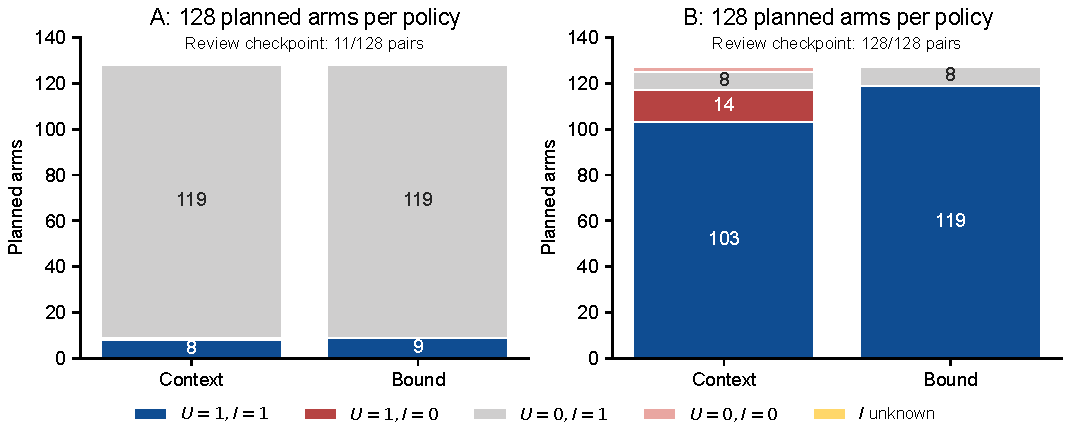
\includegraphics[width=.98\textwidth]{figures/figure2-joint-outcomes.pdf}
\caption{Original planned-ledger utility and integrity. Each policy/deployment column contains 128 arms. The large $U=0,I=1$ component in A reflects covered state with provider failures, predominantly before review. Small joint cells and both unknowns remain explicit in the main joint-outcome table and the complete table below.}
\label{fig:s-joint}
\end{figure}

\subsection{Complete scenario/configuration/policy table}
Table~\ref{tab:full-online} gives the full original denominator. Checkpoint counts refer to the shared prospective prefix. Runtime denotes the frozen exporter's prefix/runtime/audit-state failure classification; malformed model output is a separate terminal class. Counts in the rejection column are arms with at least one rejected admission, not numbers of all rejection episodes. Receipt unavailability is separately classified feedback and is not an admission rejection.
\begin{longtable}{@{}lllrrrrrrrr@{}}
\caption{Complete formal outcomes by family, deployment and policy. C=context, B=bound; CP=checkpoint reached; U=task completion; Rj=arms with rejected admission; RT=runtime failures.}\label{tab:full-online}\\
\toprule
Family & Config & Policy & Planned & CP & U & $I=1$ & $I=0$ & Unknown & Rj & RT\\
\midrule\endfirsthead
\toprule Family & Config & Policy & Planned & CP & U & $I=1$ & $I=0$ & Unknown & Rj & RT\\\midrule\endhead
E & A & B & 16 & 2 & 1 & 16 & 0 & 0 & 1 & 15 \\
E & A & C & 16 & 2 & 1 & 16 & 0 & 0 & 2 & 15 \\
E & B & B & 16 & 16 & 15 & 16 & 0 & 0 & 16 & 0 \\
E & B & C & 16 & 16 & 15 & 16 & 0 & 0 & 16 & 0 \\
G & A & B & 16 & 1 & 1 & 16 & 0 & 0 & 1 & 15 \\
G & A & C & 16 & 1 & 1 & 15 & 1 & 0 & 0 & 15 \\
G & B & B & 16 & 16 & 16 & 16 & 0 & 0 & 16 & 0 \\
G & B & C & 16 & 16 & 14 & 0 & 16 & 0 & 0 & 0 \\
L & A & B & 32 & 3 & 3 & 32 & 0 & 0 & 0 & 29 \\
L & A & C & 32 & 3 & 3 & 32 & 0 & 0 & 0 & 29 \\
L & B & B & 32 & 32 & 32 & 32 & 0 & 0 & 0 & 0 \\
L & B & C & 32 & 32 & 32 & 32 & 0 & 0 & 0 & 0 \\
N & A & B & 32 & 3 & 3 & 32 & 0 & 0 & 0 & 29 \\
N & A & C & 32 & 3 & 3 & 32 & 0 & 0 & 0 & 29 \\
N & B & B & 32 & 32 & 28 & 31 & 0 & 1 & 0 & 0 \\
N & B & C & 32 & 32 & 28 & 31 & 0 & 1 & 0 & 0 \\
R & A & B & 16 & 2 & 1 & 16 & 0 & 0 & 0 & 15 \\
R & A & C & 16 & 2 & 1 & 16 & 0 & 0 & 0 & 15 \\
R & B & B & 16 & 16 & 16 & 16 & 0 & 0 & 0 & 0 \\
R & B & C & 16 & 16 & 16 & 16 & 0 & 0 & 0 & 0 \\
V & A & B & 16 & 0 & 0 & 16 & 0 & 0 & 0 & 16 \\
V & A & C & 16 & 0 & 0 & 16 & 0 & 0 & 0 & 16 \\
V & B & B & 16 & 16 & 12 & 16 & 0 & 0 & 13 & 0 \\
V & B & C & 16 & 16 & 12 & 16 & 0 & 0 & 13 & 0 \\
\bottomrule\end{longtable}

\subsection{Primary effects and unknown identification}
The frozen aggregate completion estimator averages the two configuration-specific paired differences within each task. Bound completes 128/256 planned arms and context 126/256. The effect is 0.0078125, with task-cluster percentile interval $[-0.01953125,0.03515625]$. Configuration A has 9/128 completions under both policies, and B has 119/128 bound versus 117/128 context. B's paired effect is 0.015625 with interval $[-0.0390625,0.0703125]$. Its discordant pairs are five context-only and seven bound-only completions; the secondary exact two-sided McNemar $p$ is 0.7744140625. A has no completion-discordant pairs.

Continuity is unknown in the interrupted N pair. The aggregate bound-minus-context failure-incidence difference has no identified single point estimate: lower and upper identified endpoints are $-0.0703125$ and $-0.0625$. Their bootstrap intervals are $[-0.08203125,-0.0625]$ and $[-0.07421875,-0.05078125]$. The intervals apply to their respective endpoints; they are not a conventional interval around an imputed estimate. In A, the observed planned-ledger difference is $-0.0078125$, interval $[-0.0234375,0]$. In B, the one unknown per policy requires identification bounds. All intervals use the frozen 10,000 scenario-stratified task-cluster draws, seed 20261007.

The transition table has 261 observed authoritative transitions. All seventeen substitutions occur in G-context (A:1, B:16), pass the context policy and fail the instance oracle. These transitions satisfy the remaining evaluated guard, source and copy-forward relations. B's N arms contain thirty exact-instance transitions per policy; A's contain three per policy. A missing transition is not inferred to be a substitution.

\subsection{Feedback, absent categories and denominators}
The complete delivered-feedback table contains 99 episodes: 93 in B and six in A. All are recoverable at their recorded feedback states. B contributes G-bound16; E-context16/E-bound16; V-context13/V-bound13; R-context9/R-bound10. A contributes G-bound1; E-context2/E-bound1; R-context1/R-bound1. No delivered episode occurs in L or N. For these data each feedback-bearing arm contributes one episode, but the analysis definition permits multiple episodes and does not treat them as independent samples.

G-bound recovery succeeds in all seventeen delivered episodes. B reuses the reviewed candidate in sixteen cases; A obtains new authorization in one. E in B recovers fifteen of sixteen per policy through fresh proposal/review; V recovers twelve of thirteen per policy. R's state-confirmation endpoint occurs in nine B episodes per policy. One additional B-bound R episode ends with correct run-level completion but no recorded recovery endpoint. A has one recovered E episode per policy, with a second context E episode interrupted during recovery; its context R state-confirmation action is followed by runtime failure before accurate task completion. Thus successful intermediate repair, episode recovery and terminal task utility remain different observations.

Observed component labels comprise reuse-reviewed, reproposal, reauthorization, evidence-refresh, state-refresh and successful-confirmation-via-state, plus runtime-failure in two delivered episodes. The delivered table has zero reverify, stale-reuse, repeated-invalid, fresh-id-invalid-loop, abandon, timeout, hallucinated-success or successful-confirmation-via-receipt labels. Zero means absent under the frozen observable classifier, not that the corresponding failure is impossible. The original component arrays are preserved alongside primary path labels.

\subsection{Complete failure partition and provider coverage}
The failure ledger has 273 distinct arms: 238 runtime-failed A arms; fifteen successfully completed context arms with instance violation; two unsuccessfully completed context arms with instance violation; sixteen other unsuccessfully completed B arms with covered intact integrity; and the two unknown N arms. These disjoint classes sum to 273. B's eighteen malformed-output terminations comprise the two unsuccessful violating G-context arms and the sixteen intact-integrity failures. No proved violation occurs outside G-context.

A's 117 failed shared prefixes yield 234 failed suffix-ledger entries. Four more suffix runtime failures occur in two reached-checkpoint pairs. The raw CLI stdout archives contain 357 provider error events identifying usage-limit exhaustion across the recorded attempts. This confirms provider quota failure rather than a semantic gate rejection. The entry-time availability probe succeeded; availability during collection is an observed resource outcome. Terminal failures are not retried as new formal tasks after the quota resets. A reaches only eleven checkpoints and one G index exposure, so its recovery observations are stated with those actual denominators.

\subsection{Operational components and accounting}
Across B's 127 pairs with two suffix records, mean bound-minus-context differences are 0.070866 agent calls, 0.039370 model turns, zero authorization requests and 1.285598 seconds actual suffix time (median 0.687 seconds). G's sixteen B pairs have one extra call each, 0.9375 extra turns on average, no extra authorization requests, mean 8.844563 seconds and median 14.539 seconds extra suffix time. In A's single exposed G pair, the extra calls are a review request and a commit; the other fifteen G pairs fail before exposure.

The capped time-to-success endpoint retains all 128 pairs per deployment. B's mean paired difference is $-9.744703$ seconds overall and $-76.5275$ seconds in G. Its G median is $+14.539$ seconds. The failed context reports receive 720 seconds, accounting for the negative mean despite positive median execution friction. The raw table retains actual elapsed and capped times separately.

The provider usage records are preserved in their native components. A distinguishes input, cached input and reasoning output; B distinguishes input, cache reads and cache creation. Unreported fields remain null. Prefix usage is charged once for each of 256 pairs, then each actual suffix's usage is added separately. These observations do not supply a common currency cost. The artifact retains every native usage record rather than inventing a conversion or duplicating a prefix across arms.

\subsection{Result files and independent inspection}
The result directory contains seven primary exports:
\begin{quote}\small
\code{table1-outcomes.csv}; \code{table2-continuity.csv};\\
\code{table3-recovery.csv}; \code{table4-utility-friction.csv};\\
\code{paired-effects.csv}; \code{failure-archaeology-all-arms.csv};\\
\code{analysis-summary.json}.
\end{quote}
Derived manuscript aggregates are a separate read-only layer. The replication manifest hashes the source freeze, raw results and published tables. Reanalysis checks the master/source hashes and recomputes the independent scores before producing tables. The artifact preserves the original interruption and resume launch audits, all provider responses and the partial N state; it does not fabricate missing termination or final-state files.

\section{Supplementary quota recovery and integration requirements}
\label{app:quota-recovery}
\subsection{Separate cohort and fixed snapshot}
The primary study remains the original 128-task, two-deployment, two-policy ledger: 256 terminal pairs and 512 planned arms, including its failures and unknowns. A subsequent quota-recovery cohort selects the 117 A pairs whose original shared prefixes encountered quota exhaustion. Its separate freeze is \code{phase2-quota-recovery-v1-c41e052eb585}; its planned denominator is 117 pairs and 234 arms. Selection on the original failure state makes this a supplementary cohort with later collection conditions, rather than a replacement for the original deployment results.

The fixed GitHub handoff at commit \code{475e66f549613aaaaa62c2ec81ffdee483636c54} contains snapshot \code{research/phase2-results-snapshots/2026-10-07T021002Z/}. At 2026-10-07 02:10:02 UTC (10:10:02 Asia/Shanghai), 45 of 117 selected pairs were terminal, accounting for 90 arms; the snapshot status is PARTIAL. The remaining 72 pairs are not established as terminal by this snapshot. These collection-status counts are transcribed from the pinned \href{https://github.com/lhh666-6/auto-dete/blob/475e66f549613aaaaa62c2ec81ffdee483636c54/research/phase2-results-snapshots/2026-10-07T021002Z/snapshot-summary.json}{snapshot-summary.json}; the partial recovery records were not independently rescored in this revision. They are not completion, integrity or recovery-success results. A static snapshot does not establish that collection remains active.

\subsection{Integration gates and reporting slots}
The completed manuscript results above use only the original formal cohort. A final supplementary export can be integrated without changing that denominator or resampling its failures:
\begin{enumerate}[leftmargin=*,itemsep=3pt]
\item Preserve the original pair identifiers, all original failed attempts and the separate recovery freeze. Verify task, prompt, tool, schema, scorer and deployment provenance against the recovery manifest; document any changed provider or resource conditions.
\item Establish terminal status for all 117 selected pairs and retain every planned recovery arm, including new failures and unknown integrity. A terminal entry need not imply a complete model trajectory.
\item Recompute the independent outcomes from received responses, events and authoritative states. Report recovery-cohort checkpoint coverage, joint $(U,I)$ cells, scenario-specific transitions, actually delivered feedback, next actions, episode endpoints and friction under their own denominators.
\item Add a separately labeled supplementary result table here and, if warranted, a short paragraph in main Section 7 comparing the observed paths with the original A evidence. Any inferential procedure must follow the recovery analysis plan and preserve the selected-cohort interpretation.
\item Update the main scope paragraph and Discussion only to the strength supported by verified recovery evidence. Broader cross-deployment conclusions require adequate coverage and comparable recorded conditions.
\end{enumerate}
No partial-cohort inferential estimate or pooled replacement result is reported in this revision. The remaining dependency is the complete verified recovery ledger and its deployment/analysis provenance. Offline manuscript revision, compilation and verification of the original evidence can be completed independently of that collection.

\end{document}
